%=======================================================================
% LuminaBone — technical methods paper, formatted as an IEEE Transactions
% article (structure mirrors a standard TIM/TMI/TPAMI paper: Introduction,
% Related Work, Proposed Method, Experiments incl. Limitations, Conclusions).
% Compile on Overleaf with the IEEEtran class.
%=======================================================================
\documentclass[journal]{IEEEtran}
\usepackage{amsmath,amssymb,bm}
\usepackage{graphicx}
\usepackage{booktabs}
\usepackage[per-mode=symbol]{siunitx}
\usepackage{algorithm}
\usepackage{algpseudocode}
\usepackage[hidelinks]{hyperref}
\usepackage{cite}

\newcommand{\vn}{\bm{n}}
\newcommand{\vl}{\bm{l}}
\newcommand{\vL}{\bm{L}}
\newcommand{\vg}{\bm{g}}
\newcommand{\vX}{\bm{X}}
\newcommand{\vP}{\bm{P}}
\newcommand{\R}{\bm{R}}
\newcommand{\tvec}{\bm{t}}
\newcommand{\K}{\bm{K}}

\begin{document}

\title{Near-Field Photometric Stereo for CT-Registered Bone-Surface
Reconstruction with a Near-Coaxial Monocular Endoscope}

\author{A.~Ding,~\IEEEmembership{}
        and~others%
\thanks{Manuscript received Month DD, YYYY; revised Month DD, YYYY.}%
\thanks{A. Ding is with the (Department, Institution, City, Country)
(e-mail: andyding09@gmail.com).}%
\thanks{Digital Object Identifier XX.XXXX/XXX.XXXX.XXXXXXX}}

\markboth{IEEE Transactions (Preprint), Vol.~XX, No.~X, Month~YYYY}%
{Ding \MakeLowercase{\textit{et al.}}: Near-Field Photometric Stereo for
CT-Registered Bone-Surface Reconstruction}

\maketitle

\begin{abstract}
Photometric stereo recovers a dense field of surface normals from images of a
fixed scene under varying illumination, and is attractive for bone because it is
albedo-invariant: it infers orientation from ratios of shading rather than from
absolute brightness or texture. However, a ring of LEDs mounted around a small
endoscope is both \emph{near-field} (the light direction and intensity vary across
the field) and \emph{near-coaxial} (the lights sit only a few degrees off the
optical axis), and the classical far-field model mis-fits this geometry, integrating
the residual brightness gradient into a spurious low-frequency curvature. This paper
gives a complete, reproducible pipeline that (i)~solves the surface with a near-field
point-source model whose per-pixel light directions and inverse-square attenuation
are linearised into a per-pixel least-squares problem, (ii)~registers the
reconstruction to a preoperative CT through dual-modality fiducials, a
Perspective-$n$-Point pose, and a two-parameter affine depth calibration, and
(iii)~evaluates it by three-dimensional fiducial registration error (FRE) against CT.
On an instrumented lumbar specimen, the near-field model reconstructs three vertebral
levels to \SIrange{1.3}{1.7}{\milli\meter} FRE with four fiducials each and removes
the far-field curvature (the worst far-field level improves from \num{6.6} to
\SI{1.7}{\milli\meter}). A direct inverse-square brightness-to-range baseline is
shown to fail on textured bone, and two failure modes are reported in full. All
stages are specified at the equation level.
\end{abstract}

\begin{IEEEkeywords}
Photometric stereo, near-field illumination, surface normal measurement, endoscopy,
CT registration, Perspective-$n$-Point, fiducial registration error.
\end{IEEEkeywords}

%=======================================================================
\section{Introduction}
\IEEEPARstart{M}{easuring} the three-dimensional shape of an exposed bony surface
from a small camera is a recurring need in image-guided surgery, where the surface
must be related to a preoperative CT. Unlike multi-view stereo or
structure-from-motion, which triangulate from parallax and require surface texture
and camera motion, photometric stereo~\cite{woodham} measures a per-pixel surface
normal from a fixed viewpoint under several illuminations. It excels at fine,
dense detail and---critically for wet, low-texture bone---it is
\emph{albedo-invariant}: the normal is recovered from the relative response across
lights, so a dark patch and a bright patch of the same orientation yield the same
normal. This is precisely the property that brightness-based range estimation lacks.

The classical formulation assumes distant, parallel illumination of constant
direction. A ring of LEDs around an \SI{18}{\milli\meter} endoscope violates this in
two ways. It is \emph{near-field}: at a working distance of \SI{55}{\milli\meter} the
per-pixel light direction and the inverse-square fall-off vary across the field. It
is also \emph{near-coaxial}: with the LEDs \SI{6}{\milli\meter} off-axis, each light
is only $\approx\!\ang{6}$ from the optical axis, so the tilt-encoding lateral
component of every light vector is small. Applying the far-field model to this rig
integrates the mis-modelled brightness gradient into a systematic, low-frequency
``bowl'' that a global scale/offset cannot remove.

This paper documents a complete pipeline that addresses the geometry directly and
validates the result quantitatively against CT. The main contributions are
summarised as follows:
\begin{itemize}
\item A near-field point-source photometric-stereo solve for a near-coaxial LED
endoscope, in which per-pixel light directions and inverse-square attenuation are
linearised into a per-pixel least-squares system and iterated with a CT-anchored
depth, removing the far-field bowl (Sec.~\ref{sec:method}).
\item A per-vertebra CT-registration protocol---dual-modality fiducials, a
Perspective-$n$-Point pose, and a two-parameter affine depth calibration---that
converts the relative photometric surface into absolute CT coordinates and provides
the evaluation ground truth (Sec.~\ref{sec:reg}).
\item A controlled comparison of far-field, near-field, and inverse-square models on
the same CT-validated data, and a transparent analysis of two failure modes, which
together isolate assumed LED positions as the dominant residual error
(Sec.~\ref{sec:exp}).
\end{itemize}

%=======================================================================
\section{Related Work}
A pixel intensity $I_j$ of a surface point with unit normal $\vn$, illuminated by
light $j$ with direction $\vl_j$ and intensity $e$, obeys the reflectance model
$I_j=e\,\rho(\vn,\vl_j,\bm v)\max(\vn^{\!\top}\vl_j,0)+\varepsilon_j$, with albedo
$\rho$ and an error term $\varepsilon_j$ for shadows, noise, and inter-reflections.
Recovering $\vn$ from several such observations is photometric stereo.

\subsection{Lambertian and Non-Lambertian Photometric Stereo}
Under the Lambertian assumption Woodham~\cite{woodham} reduced the model to a linear
system solvable by least squares; the recovered gradient field is then integrated to
depth, classically by Frankot--Chellappa~\cite{fc}. Extending photometric stereo to
real, non-Lambertian materials has followed several strategies---robust
outlier-rejection methods that treat specularity and shadow as sparse anomalies,
analytic and empirical BRDF models, example-based methods, and, more recently,
learning-based networks that regress normals directly from the observations. These
approaches target the \emph{reflectance} challenge; they largely retain the
\emph{far-field} illumination assumption.

\subsection{Near-Field and LED-Based Illumination}
When the light source is close to the surface, direction and intensity vary
per-pixel. Qu\'eau et al.~\cite{queau} give a full LED forward model (position,
direction, anisotropy, fall-off) with a calibration procedure, and robust point-light
\emph{position} calibration has been reported to millimetre accuracy~\cite{aocalib}.
Accurate knowledge of the source geometry is essential in this regime, because errors
in the assumed light position propagate directly into the recovered surface---the
observation that motivates the failure analysis of this paper.

\subsection{Surgical Surface Reconstruction and Registration}
Optical reconstruction of exposed bone and its registration to CT is established with
\emph{other} modalities---notably stereovision and structured light in open
surgery---and quality is quantified by fiducial/target registration error following
Fitzpatrick et al.~\cite{fitzpatrick}, with rigid alignment via least-squares pose or
ICP. The present work targets the same registration goal from a single near-coaxial
endoscopic camera using photometric stereo, and validates it per vertebra.

%=======================================================================
\section{Proposed Method}\label{sec:method}
The pipeline has three stages: photometric-stereo depth
(Secs.~\ref{sub:sys}--\ref{sub:integrate}), CT registration (Sec.~\ref{sec:reg}),
and surface extraction (Sec.~\ref{sub:surf}). Table~\ref{tab:notation} lists notation.

\begin{table}[t]\centering
\caption{Principal notation.}\label{tab:notation}
\small
\begin{tabular}{ll}
\toprule
Symbol & Meaning\\
\midrule
$I_s(u,v)$ & linear luminance under LED $s$ at pixel $(u,v)$\\
$\vL_s,\ \vl_s$ & far-/near-field unit light direction\\
$\vn,\ \rho,\ \vg{=}\rho\vn$ & normal, albedo, photometric vector\\
$\K,\ f_x,f_y,c_x,c_y$ & intrinsics / focal lengths / principal point\\
$\R,\tvec$ & CT$\to$camera rotation, translation\\
$D(u,v)$ & metric depth from the lens (\si{\milli\meter})\\
$a,b$ & affine depth-calibration scale, offset\\
$\vP_s,\ a_r$ & LED position, ring radius\\
\bottomrule
\end{tabular}
\end{table}

\subsection{Imaging System and Image Formation}\label{sub:sys}
The endoscope (native $640\times480$) carries four LEDs on a ring of radius
$a_r=\SI{6.05}{\milli\meter}$ at azimuths \ang{0}, \ang{90}, \ang{180}, \ang{270}.
For each pose it records a dark frame and four single-LED frames. Raw sRGB frames are
converted to linear luminance in four steps: ambient subtraction
$\tilde B_s=\max(B_s-B_0,0)$; sRGB$\to$linear gamma decoding; a Rec.\,601 luminance
combination $I_s=0.299R+0.587G+0.114B$; and specular inpainting of bright,
low-saturation pixels (retroreflective glints violate Lambert). Because the four
frames are captured separately, each is divided by its median to remove per-frame
gain differences without altering intra-frame spatial variation.

\subsection{Illumination Geometry and LED Index Mapping}\label{sub:led}
At a working distance $D$ each LED subtends a half-angle
\begin{equation}
\alpha=\arctan\!\big(a_r/D\big),
\label{eq:alpha}
\end{equation}
so at $D=\SI{55}{\milli\meter}$, $\alpha\approx\ang{6.3}$: the lateral (tilt-encoding)
component of each light direction is only $\sin\alpha\approx0.11$. The mapping from
frame index to azimuth must be correct---an incorrect assignment produced normals
whose integrated depth was \emph{anti}-correlated with CT ($r\approx-0.73$), whereas
the correct wiring (LED1\,$\to$\,\ang{90}, LED2\,$\to$\,\ang{270},
LED3\,$\to$\,\ang{180}, LED4\,$\to$\,\ang{0}) gives $r\approx+0.97/{+}0.99$; the
mapping was resolved by scoring all $4!$ permutations against CT depth.

\subsection{Far-Field Photometric Stereo}\label{sub:ff}
Under distant illumination $I_s=\rho(\vn\!\cdot\!\vL_s)$ with $\vL_s$ constant over
the field. Stacking $S{=}4$ observations, $\bm I=\bm L\,\vg$ with $\vg=\rho\vn$ and
$\bm L\in\mathbb{R}^{S\times3}$, and
\begin{equation}
\hat\vg=\bm L^{+}\bm I,\qquad \rho=\lVert\vg\rVert,\qquad \vn=\vg/\lVert\vg\rVert,
\label{eq:ffsolve}
\end{equation}
with $\bm L^{+}$ the pseudo-inverse and the sign fixed so $n_z\ge0$. The albedo enters
only as the magnitude of $\vg$, giving the albedo-invariance noted above.

\subsection{Near-Field Point-Source Photometric Stereo}\label{sub:nf}
In a frame with $+x$ right, $+y$ up, $+z$ toward the camera, a pixel $(u,v)$ at metric
depth $D$ back-projects to
\begin{equation}
\vX(u,v,D)=D\Big[\tfrac{u-c_x}{f_x},\,-\tfrac{v-c_y}{f_y},\,-1\Big]^{\!\top},
\label{eq:bp}
\end{equation}
and LED $s$ sits at $\vP_s=[a_r\cos\phi_s,\,a_r\sin\phi_s,\,0]^{\!\top}$. The incident
direction and inverse-square attenuation are
\begin{equation}
\vl_s=\frac{\vP_s-\vX}{\lVert\vP_s-\vX\rVert},\qquad
w_s=\frac{1}{\lVert\vP_s-\vX\rVert^{2}}.
\label{eq:nflight}
\end{equation}
The point-source model $I_s=\rho(\vn\!\cdot\!\vl_s)w_s$ is linearised by moving the
attenuation to the observation,
\begin{equation}
m_s:=I_s\,\lVert\vP_s-\vX\rVert^{2}=\rho(\vn\!\cdot\!\vl_s)=\vg\!\cdot\!\vl_s,
\label{eq:nflin}
\end{equation}
which is linear in $\vg$ but with a \emph{per-pixel} design matrix
$\bm\Lambda=[\vl_1,\dots,\vl_S]^{\!\top}$, solved as
\begin{equation}
\hat\vg=(\bm\Lambda^{\!\top}\bm\Lambda+\epsilon\bm I)^{-1}\bm\Lambda^{\!\top}\bm m .
\label{eq:nfsolve}
\end{equation}
Because $\bm\Lambda$ and $w_s$ depend on the unknown $D$, the solve is iterated
(Algorithm~\ref{alg:nf}). LED positions $\vP_s$ are \emph{assumed} from the ring
geometry---the principal approximation of this work.

\begin{algorithm}[t]
\caption{Near-field photometric-stereo depth}\label{alg:nf}
\begin{algorithmic}[1]
\State $D\gets$ plane at $\bar D_{\text{CT}}$ (mean fiducial depth)
\For{$k=1$ to $4$}
  \State compute $\vX,\vl_s,w_s$ from $D$ via \eqref{eq:bp}--\eqref{eq:nflight}
  \State $m_s\gets I_s\lVert\vP_s-\vX\rVert^{2}$; solve $\hat\vg$ \eqref{eq:nfsolve}
  \State $\vn\gets\hat\vg/\lVert\hat\vg\rVert$, orient $n_z\ge0$
  \State $Z\gets$ integrate$(\vn)$ \eqref{eq:pq}--\eqref{eq:fc}
  \State $(a,b)\gets$ fit $D=aZ+b$ on fiducials \eqref{eq:affine}; $D\gets aZ+b$
\EndFor
\State \Return $D$
\end{algorithmic}
\end{algorithm}

\subsection{Normal Integration}\label{sub:integrate}
Depth is recovered from the normal-implied gradients
\begin{equation}
p=n_x/n_z,\qquad q=-n_y/n_z,
\label{eq:pq}
\end{equation}
by the Frankot--Chellappa least-squares-integrable solution in the frequency domain,
\begin{equation}
Z=\mathcal{F}^{-1}\!\left\{\frac{-\jmath\omega_x\hat P-\jmath\omega_y\hat Q}
{\omega_x^2+\omega_y^2}\right\},
\label{eq:fc}
\end{equation}
with the DC term zeroed (so $Z$ is relative depth) and the gradient field
even-reflected before the transform to suppress border wrap-around.

\subsection{Inverse-Square Baseline}\label{sub:invsq}
For comparison, range is also estimated directly from brightness. With
$I\propto\rho\,\Phi/r^2$,
\begin{equation}
r=\sqrt{\rho\Phi}\,/\sqrt{I}\ \Longrightarrow\ r\propto I^{-1/2},
\label{eq:invsq}
\end{equation}
which recovers range only under constant albedo---false on textured bone, where dark
pixels are read as ``far.''

\subsection{Camera Calibration and Pose}\label{sub:calib}
Intrinsics $\K$ and distortion come from a ChArUco target; the working focal length
$f_x\approx\SI{860}{px}$ is validated by four-point PnP reprojection
(\SI{0.42}{px} residual). Detection and the solve run on raw frames; distortion is
inverted analytically in projection and back-projection.

\subsection{CT Registration}\label{sec:reg}
Each retroreflective fiducial gives a pixel $\bm u_i$ (sparkle/dark-ring detection
with a $\ge3$-frame quorum) and a CT coordinate $\vX_i^{\text{CT}}$ (marker crater).
The CT$\to$camera pose of one vertebra minimises reprojection over its $N\ge4$
non-coplanar fiducials,
\begin{equation}
(\R,\tvec)=\arg\min_{\R,\tvec}\sum_{i=1}^{N}
\big\lVert\pi(\K[\R|\tvec]\vX_i^{\text{CT}})-\bm u_i\big\rVert^2,
\label{eq:pnp}
\end{equation}
solved by SQPnP~\cite{sqpnp} (globally optimal, stable at $N{=}4$). The fiducial
metric depths $z_i^{\text{CT}}=[\R\vX_i^{\text{CT}}+\tvec]_z$ fix the affine scale and
offset of the relative depth,
\begin{equation}
(a,b)=\arg\min_{a,b}\sum_{i}\big(aZ(\bm u_i)+b-z_i^{\text{CT}}\big)^2,\quad D=aZ+b,
\label{eq:affine}
\end{equation}
noting $(a,b)$ are only two scalars and cannot deform the surface. Each kept pixel is
lifted and transformed into CT coordinates,
\begin{equation}
\vX^{\text{cam}}=D\,\K^{-1}[\bm u;1],\qquad
\vX^{\text{CT}}=\R^{\!\top}(\vX^{\text{cam}}-\tvec).
\label{eq:tocT}
\end{equation}
Because the spine flexes between levels, each vertebra is registered independently.

\subsection{Surface Extraction}\label{sub:surf}
A pixel is kept if bright enough, photometrically consistent (per-pixel residual
$\varrho=\sum_s|I_s-(\hat\vg\!\cdot\!\vl_s)w_s|/\sum_s I_s<0.22$), within a depth band
about the fiducials, and not a gross spike; the border is cropped, the largest
connected components are kept, and a morphological opening removes speckle. Depth is
smoothed by normalised convolution and triangulated on the image grid, emitting a quad
only where its four corners are kept and span $<\SI{3}{\milli\meter}$.

%=======================================================================
\section{Experiments}\label{sec:exp}
\subsection{Setup and Metrics}
Five vertebral levels of one instrumented lumbar specimen were captured, each with
four fiducials (level~7: three). The primary metric is the three-dimensional fiducial
registration error,
\begin{equation}
\text{FRE}=\sqrt{\tfrac1N\textstyle\sum_i
\lVert\hat\vX_i^{\text{CT}}-\vX_i^{\text{CT,gt}}\rVert^2},
\label{eq:fre}
\end{equation}
with the reconstructed fiducial from \eqref{eq:tocT}. Residual low-frequency shape is
proxied by plane-fit deviation. Table~\ref{tab:geom} lists per-level geometry; all
levels were imaged at a similar working distance (\SIrange{51}{60}{\milli\meter}),
consistent with the measured field width at $f_x{=}\SI{860}{px}$.

\begin{table}[t]\centering
\caption{Per-level geometry. WD: working distance; $\alpha$: LED half-angle
\eqref{eq:alpha}; coplanarity: RMS fiducial out-of-plane thickness.}
\label{tab:geom}\small\sisetup{table-format=2.2}
\begin{tabular}{lcccc}
\toprule
Level & WD (mm) & $\alpha$ (\si{\degree}) & Coplanarity (mm) & \# markers\\
\midrule
4 & 60.0 & 5.8 & 0.83 & 4\\
5 & 55.4 & 6.2 & 0.14 & 4\\
6 & 58.9 & 5.9 & 0.58 & 4\\
7 & 58.6 & 5.9 & 0.00 & 3\\
8 & 51.5 & 6.7 & 1.42 & 4\\
\bottomrule
\end{tabular}
\end{table}

\subsection{Far-Field vs.\ Near-Field}
Table~\ref{tab:fre} reports the FRE. On the three well-conditioned 4-marker levels the
near-field model reaches \SIrange{1.32}{1.74}{\milli\meter}; the decisive case is
level~6, from \num{6.57} to \SI{1.74}{\milli\meter}. Fig.~\ref{fig:bowl} shows the
mechanism: with identical registration, the far-field surface bows while the
near-field surface flattens. Even on level~4 the far-field plane-fit deviation is
\SI{6.90}{\milli\meter} versus \SI{4.98}{\milli\meter} near-field (part is genuine
bone relief), confirming the bowl is a shape error the affine cannot remove.

\begin{table}[t]\centering
\caption{Three-dimensional fiducial registration error (mm).}\label{tab:fre}
\small\sisetup{table-format=1.2}
\begin{tabular}{lccl}
\toprule
Level & Far-field & Near-field & Note\\
\midrule
4 & 1.54 & 1.72 & well-conditioned\\
5 & 1.22 & 1.32 & well-conditioned\\
6 & 6.57 & \textbf{1.74} & bowl removed\\
7 & 11.14 & 9.72 & 3 markers\\
8 & 5.66 & --- & near-field diverged\\
\bottomrule
\end{tabular}
\end{table}

\begin{figure}[t]\centering
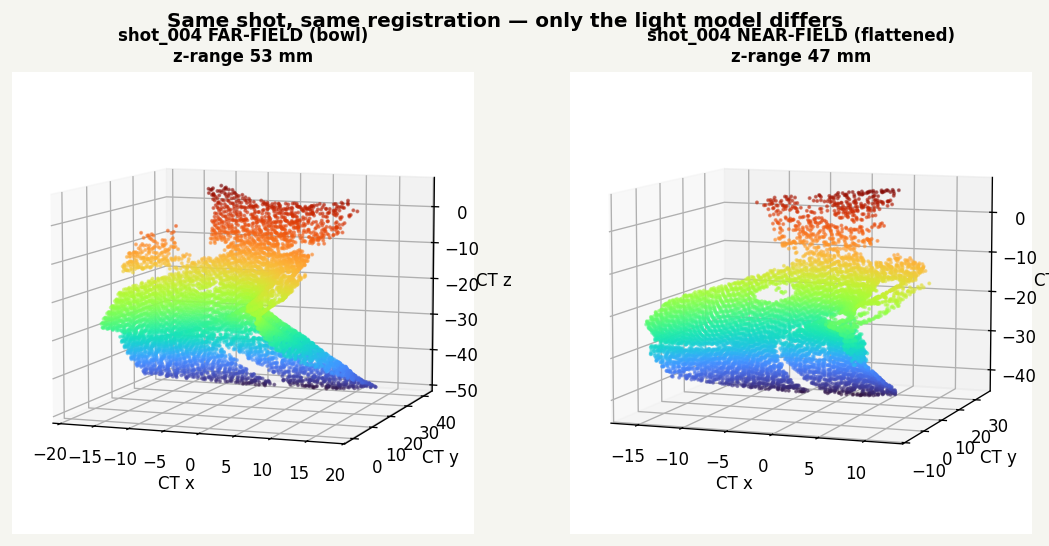
\includegraphics[width=\columnwidth]{figures/fig2_bowl.png}
\caption{Level 4, identical registration---only the light model differs. Far-field
(left) integrates a bowl; the near-field solve (right) flattens it.}
\label{fig:bowl}
\end{figure}

\begin{figure}[t]\centering
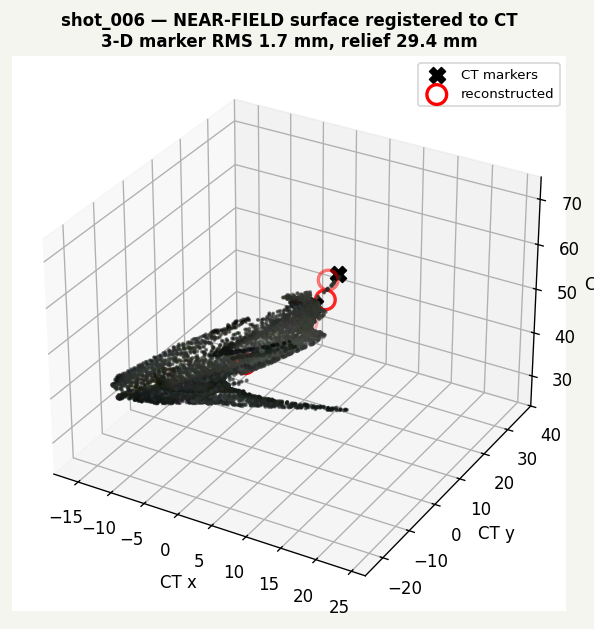
\includegraphics[width=0.86\columnwidth]{figures/fig3_shot6.png}
\caption{Level 6 near-field surface registered into CT coordinates; reconstructed
fiducials (open) on CT ground truth (crosses). FRE \SI{1.74}{\milli\meter}, versus
\SI{6.57}{\milli\meter} far-field.}
\label{fig:shot6}
\end{figure}

\subsection{Inverse-Square Baseline}
With identical CT anchoring, the inverse-square estimator~\eqref{eq:invsq} gave
\SIrange{7.8}{9.6}{\milli\meter} FRE, dense relief inflating to
\SIrange{150}{559}{\milli\meter} (true CT range \SIrange{17}{26}{\milli\meter}), and a
fitted depth slope of the wrong sign---direct consequences of the constant-albedo
assumption, quantifying why the normal-based solve is required.

\subsection{Failure Modes}
All levels are at \SIrange{51}{60}{\milli\meter}, so the two failures are not
distance-driven. Level~7 has only three fiducials, leaving the PnP
pose~\eqref{eq:pnp} under-constrained (P3P admits up to four solutions). Level~8 has
the \emph{best} marker geometry (Table~\ref{tab:geom}) yet the near-field iteration
diverged and the confidence mask collapsed, while the far-field solve stayed stable
(\SI{5.66}{\milli\meter}); this is an unresolved solver-robustness issue, reported
rather than omitted.

\subsection{Limitations}
The dominant residual error is the use of \emph{assumed} rather than calibrated LED
positions $\vP_s$; a mirror-sphere or matte-target calibration~\cite{queau,aocalib} is
the natural next step. The near-coaxial geometry ($\alpha\approx\ang{6}$)
intrinsically compresses recovered relief, since the tilt signal scales with
$\sin\alpha$. Because working distance was effectively fixed here
(\SIrange{51}{60}{\milli\meter}), its effect on accuracy could not be characterised; a
controlled distance sweep, additional specimens, repeatability, and an independent
surface-to-surface metric are the planned extensions.

%=======================================================================
\section{Conclusions and Future Work}
We have documented, at the equation level, a photometric-stereo pipeline that
reconstructs an exposed bony surface from a near-coaxial monocular endoscope and
registers it to CT. A near-field point-source solve removes the systematic bowl of the
far-field model and reconstructs three well-conditioned lumbar levels to
\SIrange{1.3}{1.7}{\milli\meter} three-dimensional FRE; an inverse-square baseline is
shown inapplicable to textured bone, and two failure modes are reported in full. Future
work will calibrate the LED positions, characterise accuracy against working distance,
and extend the validation to additional specimens with repeatability and independent
surface metrics.

\begin{thebibliography}{9}\small
\bibitem{woodham} R.~J. Woodham, ``Photometric method for determining surface
orientation from multiple images,'' \emph{Opt. Eng.}, vol.~19, no.~1, pp.~139--144,
1980.
\bibitem{fc} R.~T. Frankot and R.~Chellappa, ``A method for enforcing integrability in
shape from shading algorithms,'' \emph{IEEE Trans. Pattern Anal. Mach. Intell.},
vol.~10, no.~4, pp.~439--451, 1988.
\bibitem{queau} Y.~Qu\'eau \emph{et al.}, ``LED-based photometric stereo: modeling,
calibration and numerical solution,'' \emph{J. Math. Imaging Vis.}, vol.~60,
pp.~313--340, 2018.
\bibitem{aocalib} ``Robust point light source calibration for near-field photometric
stereo,'' \emph{Appl. Opt.}, vol.~62, no.~36, p.~9512, 2023.
\bibitem{sqpnp} G.~Terzakis and M.~Lourakis, ``A consistently fast and globally
optimal solution to the perspective-$n$-point problem,'' in \emph{Proc. ECCV}, 2020.
\bibitem{fitzpatrick} J.~M. Fitzpatrick, J.~B. West, and C.~R. Maurer, ``Predicting
error in rigid-body point-based registration,'' \emph{IEEE Trans. Med. Imag.},
vol.~17, no.~5, pp.~694--702, 1998.
\end{thebibliography}

\end{document}
